\documentclass[12pt]{article}
 
\usepackage[margin=1in]{geometry} 
\usepackage{amsmath,amsthm,amssymb}
\usepackage{listings}
\usepackage{tikz}
\usepackage{colortbl}
\usepackage{verbatim}
\usetikzlibrary{arrows, angles, quotes, decorations.pathreplacing}
\usepackage{framed}

\lstset{basicstyle=\footnotesize}
\usetikzlibrary{calc}

\newcommand{\N}{\mathbb{N}}
\newcommand{\Z}{\mathbb{Z}}
\newcommand{\I}{\mathbb{I}}
\newcommand{\R}{\mathbb{R}}
\newcommand{\Q}{\mathbb{Q}}
 
\begin{document}
 
\title{Extreme Principle\\
    \large CS101A Problem Solving I}
\author{Harry Coleman}
\date{October 22, 2019}

\maketitle

\section*{Problem 3}
\fbox{
    \parbox{\textwidth} {
        Prove that among any 50 distinct positive integers strictly less than 100 there are two that are coprime.
    }
}
\\

First, we need to show that any two consecutive integers are coprime. We will do this by a direct proof.

\begin{enumerate}
    \begin{framed}
        \item Let $x$ and $x+1$ be two arbitrary consecutive integers.
        \item $(\gcd((x+1), x) = 1) \implies x, (x+1) \text{ are coprime})$ by Definition of Coprime. 
        \item $\gcd((x+1), x) = \gcd(x, 1)$ by Euclid's Algorithm.
        \item $\gcd((x+1), x) = 1$ since $\forall a((a \in \Z) \implies (\gcd(a,1)=1))$.
        \item $x$ and $x+1$ are coprime by Definition of Coprime.
        \\\\
        Therefore, any two consecutive integers are coprime.
    \end{framed} 
\end{enumerate}

We'll use this in the main proof, which will be by contradiction. 

\begin{enumerate}
    \begin{framed}
        \item Assume it is possible to construct a set of 50 distinct positive integers strictly less than 100, such that no two are coprime.
        \item Let $S$ be such a set, ordered with $\leq$.
        \item $\forall x((x \in S) \implies x<100)$ by Definition of $S$.
        \item $\forall x\forall y(((x \in S) \land (y \in S) \land (x \ne y)) \implies (\gcd(x,y) \ne 1))$ by Definition of $S$.
        \item $1 \notin S$ since 1 is coprime with all integers.
        \item $\forall x((x \in S) \implies 2 \leq x)$ by Definition of $S$ and line 5.
        \item Let $a_n$ be the $n$th element of $S$.
        \item Let $a_1$ be the least element of $S$.
        \item $2 \leq a_1$ by line 6.
        \begin{framed}
            Subproof to show $a_n + 2 \leq a_{n+1}$ by Contradiction.
            \item Assume $a_n + 2 > a_{n+1}$.
            \item $a_n < a_{n+1}$ by Definition of $S$.
            \item $a_n < a_{n+1} < a_n + 2$ by Conjunction on lines 10, 11.
            \item $a_{n+1} = a_n + 1$ by Definition of $S$.
            \item $\gcd(a_n, a_n+1) = 1$ since any two consecutive integers are coprime.
            \item $\exists x \exists y((x\in S) \land (y \in S) \land (x \ne y) \land (gcd(x, y) = 1))$
            \item $F$ by Contradiction on lines 4, 5.
            
            Therefore, our assumption is false.
        \end{framed}
        \item  $a_n + 2 \leq a_{n+1}$ by Subproof lines 10-16.
        \item $a_1 + 2(n-1) \leq a_n$ by Definition of Arithmetic Sequence.
        \item Let $a_{50}$ be the greatest term in $S$.
        \item $2 + 2(50 -1) \leq a_{50}$ by substitution on lines 9, 18, 19.
        \item $100 \leq a_{50}$ by Arithmetic on line 20.
        \item $\exists x((x \in S) \land 100 \leq x)$ by Existential Generalization on line 21.
        \item $F$ by Contradiction on lines 3, 22.
        
        Therefore our assumption is false.
    \end{framed} 
\end{enumerate}

For any set of 50 distinct positive integers strictly less than 100, there must be at least 2 that are coprime.

\newpage
\section*{Problem 4}
\fbox{
    \parbox{\textwidth} {
        I invite 10 couples to a party at my house. I ask everyone present, including my wife, how many people they shook hands with. It turns out that everyone questioned shook hands with a different number of people. If we assume that no one shook hands with his or her partner, how many people did my wife shake hands with?
    }
}
\\

In this situation, 21 people were questioned. 10 couples and the wife of the narrator. However, we do have the narrator as a 22nd person who was shaking hands with people. Each person could have shaken hands with at most 20 people, since no one could shake hands with their partner or themselves. A person could have shaken hands with no people. Each number of shakes is a distinct non-negative integer. So we can define our set of number of handshakes in the following way.
\[S = \{0,1,2,3,4,5,6,7,8,9,10,11,12,13,14,15,16,17,18,19,20\}\]

We'll also define a function $g(x)$ where $x \in S$, which refers to the guest with that number of handshakes, but never the narrator. (Example: $g(5)$ would refer to the guest who shook hands with 5 other guests.)

Since no one shook hands with $g(0)$, we know that $g(20)$ shook hands with each of the other 20 guests. So $g(0)$ is the only guest $g(20)$ did not shake hands with. This means that $g(0)$ and $g(20)$ are a couple. We'll denote couples by a common letter.
\begin{center}
    \begin{tabular}{|c|c|c|c|c|c|c|c|c|c|c|c|c|c|c|c|c|c|c|c|c|}
        \hline
        0 & 1 & 2 & 3 & 4 & 5 & 6 & 7 & 8 & 9 & 10 & 11 & 12 & 13 & 14 & 15 & 16 & 17 & 18 & 19 & 20 \\
        A &  &  &  &  &  &  &  &  &  &  &  &  &  &  &  &  &  &  &  & A \\
        \hline
    \end{tabular}
\end{center}

Looking now at $g(19)$ and $g(1)$. $g(1)$, having shaken hands with $g(20)$, could not have shaken hands with $g(19)$. This means that $g(19)$ shook hands with everyone but $g(0)$ and $g(1)$. However, because we already know that $g(0)$ is in a couple with $g(20)$, we know that $g(1)$ and $g(19)$ are a couple.
\begin{center}
    \begin{tabular}{|c|c|c|c|c|c|c|c|c|c|c|c|c|c|c|c|c|c|c|c|c|}
        \hline
        0 & 1 & 2 & 3 & 4 & 5 & 6 & 7 & 8 & 9 & 10 & 11 & 12 & 13 & 14 & 15 & 16 & 17 & 18 & 19 & 20 \\
        A & B &  &  &  &  &  &  &  &  &  &  &  &  &  &  &  &  &  & B & A \\
        \hline
    \end{tabular}
\end{center}

Similarly, $g(18)$ must have shaken hands with everyone except for $g(0)$, $g(1)$, and $g(2)$. Since $g(0)$ and $g(1)$ are in couples with $g(20)$ and $g(19)$, respectively, $g(18)$ must be in a couple with $g(2)$.
\begin{center}
    \begin{tabular}{|c|c|c|c|c|c|c|c|c|c|c|c|c|c|c|c|c|c|c|c|c|}
        \hline
        0 & 1 & 2 & 3 & 4 & 5 & 6 & 7 & 8 & 9 & 10 & 11 & 12 & 13 & 14 & 15 & 16 & 17 & 18 & 19 & 20 \\
        A & B & C &  &  &  &  &  &  &  &  &  &  &  &  &  &  &  & C & B & A \\
        \hline
    \end{tabular}
\end{center}

We can see how this pattern would continue until the parings reach the center of the list.
\begin{center}
    \begin{tabular}{|c|c|c|c|c|c|c|c|c|c|c|c|c|c|c|c|c|c|c|c|c|}
        \hline
        0 & 1 & 2 & 3 & 4 & 5 & 6 & 7 & 8 & 9 & 10 & 11 & 12 & 13 & 14 & 15 & 16 & 17 & 18 & 19 & 20 \\
        A & B & C & D & E & F & G & H & I & J &  & J & I & H & G & F & E & D & C & B & A \\
        \hline
    \end{tabular}
\end{center}

Since $g(10)$ is not in a couple with anyone in our set, they must be in a couple with the narrator, the only individual not in the set. The wife shook hands with 10 people.
 

\section*{Problem 5}
\fbox{
    \parbox{\textwidth} {
        Seven dwarfs are sitting around a circular table. There is a cup in front of each. There is milk in some cups, altogether 3 liters. One of the dwarfs shares his milk uniformly with the other cups. Proceeding counter-clockwise, each of the other dwarfs, in turn, does the same. After the seventh dwarf has shared his milk, the initial content of each cup is restored. Find the initial amount of milk in each cup.

    }
}
\\

We'll define our set of dwarfs' cups' milk quantities as
\[S_0 = \{A_0, B_0, C_0, D_0, E_0, F_0, G_0\}\]

Where $A$ is the first dwarf around the table, $B$ the second, and so on. And the subscript 0 denotes the initial quantities. For the first round of sharing, $A$ empties their cup of milk equally into each of the other dwarfs' cups, leaving $A$ with none. After this, we have
\[S_1 = \{B_1, C_1, D_1, E_1, F_1, G_1, A_1\}\]

where
\[B_1 = B_0 + (A_0/6)\]
\[C_1 = C_0 + (A_0/6)\]
\[D_1 = D_0 + (A_0/6)\]
\[E_1 = E_0 + (A_0/6)\]
\[F_1 = F_0 + (A_0/6)\]
\[G_1 = G_0 + (A_0/6)\]
\[A_1 = 0\]

Similarly, for the second round of sharing, $B$ empties their cup of milk equally into each of the other dwarfs' cups, leaving $B$ with none. So
\[S_2 = \{C_2, D_2, E_2, F_2, G_2, A_2, B_2\}\]

where
\[C_2 = C_1 + (B_1/6)\]
\[D_2 = D_1 + (B_1/6)\]
\[E_2 = E_1 + (B_1/6)\]
\[F_2 = F_1 + (B_1/6)\]
\[G_2 = G_1 + (B_1/6)\]
\[A_2 = A_1 + (B_1/6)\]
\[B_2 = 0\]

This continues until the seventh dwarf, $G$, has shared their milk. Which brings us back to our initial amounts.
\[S_7 = \{A_0, B_0, C_0, D_0, E_0, F_0, G_0\}\]

This also has the result that if we were to continue the process past a full cycle, we would find that
\[S_8 = \{B_1, C_1, D_1, E_1, F_1, G_1, A_1\}\]
\[S_9 = \{C_2, D_2, E_2, F_2, G_2, A_2, B_2\}\]
and so on. This means that the property of $S_0$ to repeat after 7 milk sharing rounds is also true of $S_1$ and $S_2$ and so on. This means that a set of values which works for $S_0$, also works for $S_1$. So we'll look at the case where $S_0$ and $S_1$ are equivalent sets.

\[S_0 = \{A_0, B_0, C_0, D_0, E_0, F_0, G_0\}\]
\[S_1 = \{B_1, C_1, D_1, E_1, F_1, G_1, A_1\}\]
\begin{align*}
    B_1 &= A_0 = B_0 + (A_0/6) \\
    C_1 &= B_0 = C_0 + (A_0/6) \\
    D_1 &= C_0 = D_0 + (A_0/6) \\
    E_1 &= D_0 = E_0 + (A_0/6) \\
    F_1 &= E_0 = F_0 + (A_0/6) \\
    G_1 &= F_0 = G_0 + (A_0/6) \\
    A_1 &= G_0 = 0
\end{align*}

Some arithmetic, and we get

\begin{align*}
    G_0 &= 0 \\
    F_0 &= \frac{1}{6} A_0 \\
    E_0 &= \frac{2}{6} A_0 \\
    D_0 &= \frac{3}{6} A_0 \\
    C_0 &= \frac{4}{6} A_0 \\
    B_0 &= \frac{5}{6} A_0
\end{align*}

Since the total amount of milk is 3 liters, we have

\[A_0 + B_0 + C_0 + D_0 + E_0 + F_0 + G_0 = 3\] 
\[A_0 + \frac{5}{6} A_0 + \frac{4}{6} A_0 + \frac{3}{6} A_0 + \frac{2}{6} A_0 + \frac{1}{6} A_0 + 0 = 3\]
\[A_0 = \frac{6}{7}\]

\[S = \left\{\frac{6}{7}, \frac{5}{7}, \frac{4}{7}, \frac{3}{7}, \frac{2}{7}, \frac{1}{7}, 0\right\}\]

Again, however, this is only one solution, there is not necessarily only one solution.


\section*{Problem 6}
\fbox{
    \parbox{\textwidth} {
         The Sikinian Parliament consists of one house. Every member has three enemies at most among the remaining members. Show that one can split the house into two houses so that every member has one enemy at most in his house.
    }
}
\\

We'll define a set of all $n$ members in the Sikinian Parliament.

\[P = \{x_1, x_2, x_3, \dots, x_n\}\]
where each $x_i$ is a member of parliament. We want to split this set into two houses, or subsets $A$ and $B$ where
\[P = A \cup B\]
\[A \subseteq P\]
\[B \subseteq P\]

We also have the property that each member of parliament has at most 3 enemies, which are also members of parliament. We will interpret the enemy relation between two members as going both ways. That is, given two members $x$ and $y$, we know that $x$ is an enemy of $y$, iff $y$ is an enemy of $x$. We'll represent this relation with the predicate
\[R(x,y) = \text{$x$ and $y$ are enemies}\]

In addition to this, we'll also define an enemy counting function on members of parliament, $E(x)$ where $x \in P$, which returns the number of enemies of $x$ in it's current subset of $P$. This means that if $x \in A$, $E(x)$ returns the number of enemies of $x$ in $A$. Likewise if $x \in B$, $E(x)$ returns the number of enemies of $x$ in $B$. Essentially, we want to show that for any Parliament $P$, we can find a partition of $P$ into $A$ and $B$ such that

\[\forall x ((x \in P) \implies (E(x) \leq 1))\]

To start, we'll take our arbitrary parliament $P$ and randomly split up the members into $A$ and $B$. So, for instance, we might have

\[A = \{x_1, x_2, x_4, \dots, x_{n-1}\}\]
\[B = \{x_3, x_5, x_6, \dots, x_n\}\]
but it does not matter specifically how the elements are split up, just some arbitrary partitioning. Every element of each set has either 0, 1, 2, or 3 enemies in the same subset as itself, or
\[\forall x((x \in P) \implies (E(x) \in \{0,1,2,3\}))\]

We don't need to immediately worry about those members with 0 or 1 enemy in the same subset, however, those members with 2 or 3 enemies in the same subset are not where we want them to be. For each of these members, we will want to swap them to the opposite set. For instance, if we have the case where
\[A = \{a, b, c, \dots\}, B = \{d, \dots\}\]
and 
\[R(a, b) \land R(a, c) \land R(a, d)\]
We would know that $E(a) = 2$. 

We'll define a function $T_t$ which returns the sum of all of the enemy counting functions, applied to all members of parliament at time $t$.

\[T_t = \sum_{x \in P}E(x)\]

We'll now look back at our set and see that $a$ is currently in a subset with two of its enemies, so we want to swap it over to the other set. After this operation, we are now at time $t=1$. The subsets at each time step are shown below.

\[A_0 = \{a, b, c, \dots\}\]
\[B_0 = \{d, \dots\}\]

\[A_1 = \{b, c, \dots\}\]
\[B_1 = \{a, d, \dots\}\]

We now want to look at how this operation affected our $T$ value from $T_0$ to $T_1$. Beginning with $a$, we see that it moved from a subset with 2 of its enemies, to a subset with only one of its enemies. So $E(a)$ decreased by 1. We can also see that removing member $a$ from $A$ decreased both $E(b)$ and $E(c)$ by 1. However, moving $a$ into $B$ increased $E(d)$ by 1. Since $a$ is only related to $b$, $c$, and $d$, no other $E(x)$ values changed. So we know that

\[T_1 = T_0 - 1 - 1 - 1 + 1 = T_0 - 2\]

So in the case that a member $x$ has $E(x) = 2$, we can decrease the overall $T$ by moving $x$ to the opposite subset. This can also easily be shown for $E(x) = 3$. Given

\[A_0 = \{a, b, c, d\dots\}\]
\[B_0 = \{\dots\}\]
where \[R(a, b) \land R(a, c) \land R(a, d)\]. We would have $E(a) = 3$. So moving $a$ to the other subset.
\[A_1 = \{b, c, d\dots\}\]
\[B_1 = \{a, \dots\}\]

Now with $E(a)=0$ and each of $E(b), E(c), E(d)$ decreasing by 1. $T_1 = T_0 - 6$. And we can continue applying this operation to any member with $E(x) > 1$ and continue to decrease $T$. And since $T$ is a sum of $E(x)$ values and $E(x)$ is non-negative, the process must stop eventually. So through successive applications, we must reach a state where 
\[\forall x ((x \in P) \implies (E(x) \leq 1))\]



%\section*{Problem 7}
%\fbox{
%    \parbox{\textwidth} {
%         Given finitely many squares whose areas add up to 1, show that they can be arranged without overlaps inside a square of area 2.
%    }
%}
%\\

\newpage
\section*{Problem 8}
\fbox{
    \parbox{\textwidth} {
         Let B and W be finite sets of black and white points, respectively, in the plane, with the property that every line segment that joins two points of the same color contains a point of the other color. Prove that both sets must lie on a single line segment.
    }
}
\\

We'll first assume that the sets do not lie on a single line segment. Since it doesn't make sense to talk about either of the sets being empty, we'll assume they are both nonempty. This means there must exist at least one black point and one white point.

\begin{center}
    \begin{tikzpicture}
        \coordinate (A) at (0, 0);
        \coordinate (B) at (4, 0);
        
        \filldraw[black] (A) circle (2pt) node[anchor=east] {$B$};
        \filldraw[black] (B) circle (2pt) node[anchor=west] {$W$};
        
        \draw[dashed] (A) -- (B);

    \end{tikzpicture}
\end{center}

If there were only these two points, they would lie on the show line segment, so there is at least one other point, black or white, that is not collinear with these two points. We'll take it to be a black point. (This could be repeated swapping all instances of black and white to show the same thing).

\begin{center}
    \begin{tikzpicture}
        \coordinate (A) at (0, 0);
        \coordinate (B) at (4, 0);
        \coordinate (C) at (3, 3);
        
        \filldraw[black] (A) circle (2pt) node[anchor=east] {$B$};
        \filldraw[black] (B) circle (2pt) node[anchor=west] {$W$};
        \filldraw[black] (C) circle (2pt) node[anchor=south] {$B$};
        
        \draw[dashed] (A) -- (C);

    \end{tikzpicture}
\end{center}

With this new black point, by the definition of our sets, there must be a white point on the shown segment between the two black points.

\begin{center}
    \begin{tikzpicture}
        \coordinate (A) at (0, 0);
        \coordinate (B) at (4, 0);
        \coordinate (C) at (3, 3);
        \coordinate (D) at (1.5, 1.5);
        
        \filldraw[black] (A) circle (2pt) node[anchor=east] {$B$};
        \filldraw[black] (B) circle (2pt) node[anchor=west] {$W$};
        \filldraw[black] (C) circle (2pt) node[anchor=south] {$B$};
        \filldraw[black] (D) circle (2pt) node[anchor=south east] {$W$};
        
        \draw[dashed] (B) -- (D);

    \end{tikzpicture}
\end{center}

With this new white point, by the definition of our sets, there must be a black point on the shown segment between the two white points.

\begin{center}
    \begin{tikzpicture}
        \coordinate (A) at (0, 0);
        \coordinate (B) at (4, 0);
        \coordinate (C) at (3, 3);
        \coordinate (D) at (1.5, 1.5);
        \coordinate (E) at (2.75, 0.75);
        
        \filldraw[black] (A) circle (2pt) node[anchor=east] {$B$};
        \filldraw[black] (B) circle (2pt) node[anchor=west] {$W$};
        \filldraw[black] (C) circle (2pt) node[anchor=south] {$B$};
        \filldraw[black] (D) circle (2pt) node[anchor=south east] {$W$};
        \filldraw[black] (E) circle (2pt) node[anchor=west] {$B$};
        
        \draw[dashed] (A) -- (C) -- (E) -- (A);

    \end{tikzpicture}
\end{center}

So there must exist at least 3 not collinear black points, which can be connected to form a triangle. With this, we'll define $T$ to be the set of the perimeters of all possible triangles constructed using 3 black points, And order this set with $\leq$. Now, we will look at the smallest of the elements in $T$, and find the points which form the triangle of minimum perimeter.

\begin{center}
    \begin{tikzpicture}
        \coordinate (A) at (0, 0);
        \coordinate (B) at (4, 0);
        \coordinate (C) at (3, 3);
        
        \filldraw[black] (A) circle (2pt) node[anchor=east] {$B$};
        \filldraw[black] (B) circle (2pt) node[anchor=west] {$B$};
        \filldraw[black] (C) circle (2pt) node[anchor=south] {$B$};
        
        \draw[dashed] (A) -- (B) -- (C) -- (A);
    \end{tikzpicture}
\end{center}

Given the property of our sets that every line segment that joins two points of the same colors contains a point of the other color, we know that each of these segments must contain a white point.

\begin{center}
    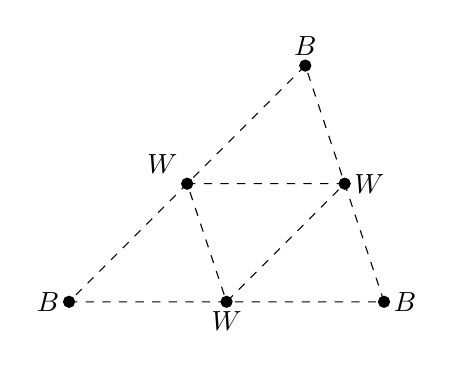
\begin{tikzpicture}
        \coordinate (A) at (0, 0);
        \coordinate (B) at (4, 0);
        \coordinate (C) at (3, 3);
        \filldraw[black] (A) circle (2pt) node[anchor=east] {$B$};
        \filldraw[black] (B) circle (2pt) node[anchor=west] {$B$};
        \filldraw[black] (C) circle (2pt) node[anchor=south] {$B$};
        
        \draw[dashed] (A) -- (B) -- (C) -- (A);
        
        \coordinate (D) at (1.5, 1.5);
        \coordinate (E) at (3.5, 1.5);
        \coordinate (F) at (2, 0);
        \filldraw[black] (D) circle (2pt) node[anchor=south east] {$W$};
        \filldraw[black] (E) circle (2pt) node[anchor=west] {$W$};
        \filldraw[black] (F) circle (2pt) node[anchor=north] {$W$};
        
        \draw[dashed] (D) -- (E) -- (F) -- (D);
        
    \end{tikzpicture}
\end{center}

Using the same property, we know that there are black points on each of these new line segments.

\begin{center}
    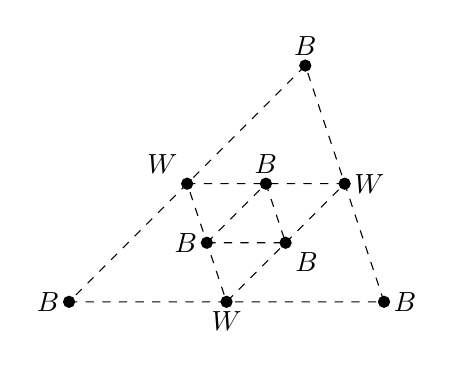
\begin{tikzpicture}
        \coordinate (A) at (0, 0);
        \coordinate (B) at (4, 0);
        \coordinate (C) at (3, 3);
        \filldraw[black] (A) circle (2pt) node[anchor=east] {$B$};
        \filldraw[black] (B) circle (2pt) node[anchor=west] {$B$};
        \filldraw[black] (C) circle (2pt) node[anchor=south] {$B$};
        
        \draw[dashed] (A) -- (B) -- (C) -- (A);
        
        \coordinate (D) at (1.5, 1.5);
        \coordinate (E) at (3.5, 1.5);
        \coordinate (F) at (2, 0);
        \filldraw[black] (D) circle (2pt) node[anchor=south east] {$W$};
        \filldraw[black] (E) circle (2pt) node[anchor=west] {$W$};
        \filldraw[black] (F) circle (2pt) node[anchor=north] {$W$};
        
        \draw[dashed] (D) -- (E) -- (F) -- (D);
        
        \coordinate (G) at (1.75, 0.75);
        \coordinate (H) at (2.5, 1.5);
        \coordinate (I) at (2.75, 0.75);
        \filldraw[black] (G) circle (2pt) node[anchor=east] {$B$};
        \filldraw[black] (H) circle (2pt) node[anchor=south] {$B$};
        \filldraw[black] (I) circle (2pt) node[anchor=north west] {$B$};
        
        \draw[dashed] (G) -- (H) -- (I) -- (G);
        
    \end{tikzpicture}
\end{center}

We have shown that there exists a smaller triangle,with a lesser perimiter, than our original one, which we defined to be the triangle of minimum perimeter among black points. So we have a contradiction, and our assumption is false. Therefore, our sets would have to all be collinear, and thus lie on a single line segment.

\section*{Problem 9}
\fbox{
    \parbox{\textwidth} {
         Consider finitely many points in the plane such that, if we choose any three points A,B,C among them, the area of triangle ABC is always less than 1. Show that all these points lie within the interior or on the boundary of a triangle with area less than 4.
    }
}
\\

We'll define $S$ to be the set of all possible areas of triangles formed by 3 points in the plane. We'll look at the triangle with the greatest area. If there are multiple triangles with the same greatest area, we can look at an arbitrary one from that group.

\begin{center}
    \begin{tikzpicture}
        \coordinate (A) at (0, 0);
        \coordinate (B) at (4, 0);
        \coordinate (C) at (3, 3);
        \filldraw[black] (A) circle (2pt) node[anchor=east] {$A$};
        \filldraw[black] (B) circle (2pt) node[anchor=west] {$B$};
        \filldraw[black] (C) circle (2pt) node[anchor=south] {$C$};
        
        \draw[black] (A) -- (B) -- (C) -- (A);
        
        \draw[dashed] (C) -- (3,0) node[anchor=east, midway] {$h$};
        \draw (2,0) node[anchor=north] {$b$};
    \end{tikzpicture}
\end{center}

The area of this maximum area triangle would be
\[\frac{1}{2}bh < 1\]

Since it is the maximum area for triangles in our set, we know there are no triangles with the same base and a greater height. So there are no points above the shown line, since any points above this line would form a triangle with $A$ and $B$ with the same base, but a greater height, and therefore a greater area than triangle $ABC$.

\begin{center}
    \begin{tikzpicture}
        \coordinate (A) at (0, 0);
        \coordinate (B) at (4, 0);
        \coordinate (C) at (3, 3);
        \filldraw[black] (A) circle (2pt) node[anchor=east] {$A$};
        \filldraw[black] (B) circle (2pt) node[anchor=west] {$B$};
        \filldraw[black] (C) circle (2pt) node[anchor=south] {$C$};
        
        \draw[black] (A) -- (B) -- (C) -- (A);
        
        \draw[dashed] (C) -- (3,0) node[anchor=east, midway] {$h$};
        \draw (2,0) node[anchor=north] {$b$};
        
        \draw[dashed] (-2,3) -- (8,3);
        
    \end{tikzpicture}
\end{center}

The line passing through $C$ is parallel to segment $AB$. The same can be done when taking $AC$ as the base, and likewise for $BC$.

\begin{center}
    \begin{tikzpicture}
        \coordinate (A) at (0, 0);
        \coordinate (B) at (4, 0);
        \coordinate (C) at (3, 3);
        \filldraw[black] (A) circle (2pt) node[anchor=east] {$A$};
        \filldraw[black] (B) circle (2pt) node[anchor=west] {$B$};
        \filldraw[black] (C) circle (2pt) node[anchor=south] {$C$};
        
        \draw[black] (A) -- (B) -- (C) -- (A);
        
        \coordinate (c1) at (-2,3);
        \coordinate (c2) at (8,3);
        
        \coordinate (b1) at (8,4);
        \coordinate (b2) at (0,-4);
        
        \coordinate (a1) at (1.33, -4);
        \coordinate (a2) at (-1.33, 4);
        
        \draw[dashed] (c1) -- (c2);
        \draw[dashed] (b1) -- (b2);
        \draw[dashed] (a1) -- (a2);
        
        \coordinate (ap) at (7,3);
        \coordinate (bp) at (-1,3);
        \coordinate (cp) at (1,-3);
        
        \filldraw[black] (ap) circle (2pt) node[anchor=north] {$A^\prime$};
        \filldraw[black] (bp) circle (2pt) node[anchor=north east] {$B^\prime$};
        \filldraw[black] (cp) circle (2pt) node[anchor=east] {$C^\prime$};
    \end{tikzpicture}
\end{center}

All the points must lie in or on triangle $A^\prime B^\prime C^\prime$. Using a few geometric identities, we can say more about this triangle. Since
\[AC \parallel BA^\prime\]
\[AB \parallel CA^\prime\]
we have parallelogram $ACA^\prime B$. So $AB \cong CA^\prime$. And using this same reasoning we can find the following congruences.

\begin{center}
    \begin{tikzpicture}
        \coordinate (A) at (0, 0);
        \coordinate (B) at (4, 0);
        \coordinate (C) at (3, 3);
        \filldraw[black] (A) circle (2pt) node[anchor=east] {$A$};
        \filldraw[black] (B) circle (2pt) node[anchor=west] {$B$};
        \filldraw[black] (C) circle (2pt) node[anchor=south] {$C$};
        
        \draw[black] (A) -- (B) -- (C) -- (A);
        
        \coordinate (c1) at (-2,3);
        \coordinate (c2) at (8,3);
        
        \coordinate (b1) at (8,4);
        \coordinate (b2) at (0,-4);
        
        \coordinate (a1) at (1.33, -4);
        \coordinate (a2) at (-1.33, 4);
        
        \draw[dashed] (c1) -- (c2);
        \draw[dashed] (b1) -- (b2);
        \draw[dashed] (a1) -- (a2);
        
        \coordinate (ap) at (7,3);
        \coordinate (bp) at (-1,3);
        \coordinate (cp) at (1,-3);
        
        \filldraw[black] (ap) circle (2pt) node[anchor=north] {$A^\prime$};
        \filldraw[black] (bp) circle (2pt) node[anchor=north east] {$B^\prime$};
        \filldraw[black] (cp) circle (2pt) node[anchor=east] {$C^\prime$};
        
        \draw (A)--(B) node[midway, rotate=-10]{$|$};
        \draw (bp)--(C) node[midway, rotate=-10]{$|$};
        \draw (C)--(ap) node[midway, rotate=-10]{$|$};
        
        \draw (A)--(C) node[midway, rotate=35]{$||$};
        \draw (cp)--(B) node[midway, rotate=35]{$||$};
        \draw (B)--(ap) node[midway, rotate=35]{$||$};
        
        \draw (B)--(C) node[midway, rotate=100]{$|||$};
        \draw (cp)--(A) node[midway, rotate=100]{$|||$};
        \draw (A)--(bp) node[midway, rotate=100]{$|||$};
    \end{tikzpicture}
\end{center}

This tells us that triangle $A^\prime B^\prime C^\prime$ is similar to $ABC$ with a linear scale factor of 2. Meaning the area of triangle $A^\prime B^\prime C^\prime$ is 4 times that of triangle $ABC$. And since the area of triangle $ABC$ is less than 1, the area of triangle $A^\prime B^\prime C^\prime$ is less than 4. So with the given conditions, all the points in our plane are on or in a triangle with an area less than 4.


\newpage
\section*{Problem 10}
\fbox{
    \parbox{\textwidth} {
         In some country all roads between cities are one-way and such that once you leave a city you cannot return to it again. Prove that there exists a city into which all roads enter and a city from which all roads exit.
    }
}
\\

First, we'll assume that there is a finite number of cities $n$ and that every city has at least one road which enters the city and at least one road which exits the city.. So we have a set of cities
\[C = \{a_1, a_2, \dots, a_n\}\]

We'll define two functions $s(x)$, the successor function, and $p(x)$, the predecessor function.

Given some city $x \in C$, $s(x)$ returns another city $y \in C$ such that there exists a road from $x$ to $y$. Since every city has at least one road which exits, we know this will always return another city. If $x$ has multiple roads which exit, it returns a random city $y \in C$ from the set of cities which have a roads from $x$. $p(x)$, by a similar process, returns another city $y \in C$ such that there exists a road from $y$ to $x$. 

For example,

\begin{center}
    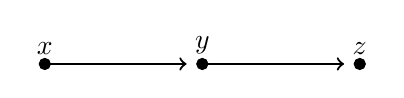
\begin{tikzpicture}
        \coordinate (A) at (0, 0);
        \coordinate (B) at (2, 0);
        \coordinate (C) at (4, 0);
        \filldraw[black] (A) circle (2pt) node[anchor=south] {$x$};
        \filldraw[black] (B) circle (2pt) node[anchor=south] {$y$};
        \filldraw[black] (C) circle (2pt) node[anchor=south] {$z$};
        
        
        \draw[->, thick] (A) -- (1.8,0);
        \draw[->, thick] (B) -- (3.8,0);
        
    \end{tikzpicture}
\end{center}

If $x,y,z \in C$
\[s(y) = z\]
\[p(y) = x\]

Taking some arbitrary city $b_0 \in C$, and knowing that it is not possible to return to a city once left, we can apply our successor function to get 
\[s(b_0) = b_1 \in C \text{ where } b_0 \ne b_1\]
And again on $b_1$ to get
\[s(b_1) = b_2 \in C \text{ where } b_0 \ne b_2 \text{ and } b_1 \ne b_2\]
And so on until
\[s(b_n-1) = b_n \in C \text{ where } b_n \notin \{b_0,\dots,b_{n-1}\}\]

This gives us $n+1$ distinct cities in our country. However, this contradicts our assumption that there are only a finite $n$ cities in $C$. So there is some city which has no successor, which would be a city into which all roads enter, and none exit. 

For the second part of the problem, we will take an arbitrary city $b_0 \in C$, this time applying the predecessor function to get
\[p(b_0) = b_{-1} \in C \text{ where } b_0 \ne b_{-1}\]
And again on $b_{-1}$ to get
\[p(b_{-1}) = b_{-2} \in C \text{ where } b_0 \ne b_{-2} \text{ and } b_{-1} \ne b_{-2}\]
And so on until
\[p(b_{-(n-1)}) = b_{-n} \text{ where } b_{-n} \notin \{b_0,\dots,b_{-(n-1)}\}\]

This gives us $n+1$ distinct cities in our country. However, this contradicts our assumption that there are only a finite $n$ cities in $C$. So there is some city which has no predecessor, which would be a city from which all roads exit, and none enter. 


\end{document}